\section{Gestión de la Cadena de Suministro con IA en la Maquiladora}

\subsection{Introducción}

La gestión eficiente de la cadena de suministro es uno de los elementos clave para el éxito de la maquiladora. El uso de \textbf{Inteligencia Artificial (IA)} en esta área permite optimizar procesos fundamentales, como la gestión de inventarios y la logística, ayudando a reducir costos, mejorar la eficiencia y aumentar la competitividad. Este capítulo presenta un análisis detallado de cómo la IA puede transformar la cadena de suministro en la industria maquiladora.

\subsubsection{Gestión de la Cadena de Suministro con IA}

El segundo proyecto se enfoca en la aplicación de IA en la gestión de la cadena de suministro. Esta solución tiene un impacto significativo en áreas clave como la \textbf{optimización de inventarios} y la \textbf{logística inteligente}, con beneficios en reducción de costos y mejora de la agilidad operativa.

\subsubsection{Ranking de Adaptación}

El siguiente ranking describe los factores clave para la implementación de IA en la gestión de la cadena de suministro:

\begin{table}[H]
\centering
\caption{Ranking de Adaptación del Proyecto 2}
\resizebox{\textwidth}{!}{
\begin{tabular}{@{}>{\bfseries}l*{5}{>{\centering\arraybackslash}p{2cm}}@{}}
\toprule
Factor & Complejidad Técnica & Tiempo de Implementación & Inversión Económica & Capacitación del Personal & Impacto en la Cultura Organizacional \\ \midrule
Valor & Medio (3) & Medio (3) & Medio (3) & Bajo (1) & Medio (3) \\ \bottomrule
\end{tabular}}
\end{table}

\subsubsection{Aplicaciones}

La IA en la gestión de la cadena de suministro tiene aplicaciones claras que ofrecen beneficios inmediatos en áreas como la optimización de inventarios y la logística. A continuación, se detallan estas aplicaciones y sus respectivos beneficios.

\subsubsection{Optimización de Inventarios}

Una de las principales preocupaciones en la cadena de suministro es el manejo eficiente de los inventarios. Con IA, las maquiladoras pueden predecir la demanda futura con mayor precisión, lo que ayuda a evitar tanto el exceso de stock (que genera costos de almacenamiento innecesarios) como la falta de stock (que puede interrumpir la producción).

\subsubsection{Beneficios}

\begin{itemize}
    \item \textbf{Reducción de costos de almacenamiento}: Mantener solo el inventario necesario, evitando excesos.
    \item \textbf{Mejora de la disponibilidad de productos}: Minimiza las interrupciones en la producción causadas por falta de insumos.
    \item \textbf{Mayor eficiencia en la cadena de suministro}: Flujo constante de materiales y productos, optimizando tiempos y recursos.
\end{itemize}

\subsubsection{Tecnologías Clave}

\begin{itemize}
    \item \textbf{Algoritmos de Predicción}: Utilizan datos históricos de demanda para predecir las necesidades futuras. Ejemplos incluyen Regresión Lineal y Redes Neuronales Recurrentes (RNNs).
    \item \textbf{Plataformas de Gestión de Inventarios}: Integran las predicciones de IA para optimizar los niveles de inventario en tiempo real.
    \item \textbf{Sensores IoT para Inventarios}: Estos sensores permiten monitorear continuamente los niveles de stock, proporcionando datos en tiempo real para decisiones más precisas.
\end{itemize}

\subsection{Logística Inteligente}

La logística en la maquiladora también puede beneficiarse considerablemente con la aplicación de IA. Los algoritmos de optimización permiten seleccionar las rutas de transporte más eficientes, programar envíos de manera óptima y realizar ajustes en tiempo real según las condiciones del mercado o la producción.

\subsubsection{Beneficios}

\begin{itemize}
    \item \textbf{Reducción de costos de transporte}: Optimización de rutas y programación de envíos más eficientes.
    \item \textbf{Mejora en los tiempos de entrega}: Capacidad para prever problemas logísticos y ajustar operaciones en tiempo real.
    \item \textbf{Mayor agilidad y capacidad de respuesta}: Respuesta rápida a cambios inesperados en la demanda o en el mercado.
\end{itemize}

\subsubsection{Tecnologías Clave}

\begin{itemize}
    \item \textbf{Algoritmos de Optimización de Rutas}: Encuentran las rutas más rápidas y económicas para el transporte de mercancías, considerando factores como el tráfico o las condiciones climáticas.
    \item \textbf{Sistemas de Gestión de Transporte (TMS)}: Utilizan IA para optimizar la planificación y ejecución del transporte, ajustando rutas y entregas en tiempo real.
    \item \textbf{Plataformas de Análisis Predictivo}: Analizan datos históricos y en tiempo real para anticipar problemas y mejorar las decisiones logísticas.
\end{itemize}

\subsubsection{Tabla Resumen de Aplicaciones y Beneficios}

A continuación, se presenta una tabla resumen de las principales aplicaciones de IA en la gestión de la cadena de suministro y sus beneficios asociados.

\begin{table}[H]
\centering
\caption{Aplicaciones de IA en la Cadena de Suministro}
\resizebox{\textwidth}{!}{
\begin{tabular}{@{}>{\bfseries}l*{3}{>{\raggedright\arraybackslash}p{4cm}}@{}}
\toprule
Aplicación & Beneficios & Tecnologías Clave \\ \midrule
Optimización de Inventarios & Reducción de costos de almacenamiento, mejora de la disponibilidad de productos, mayor eficiencia en la cadena de suministro & Algoritmos de Predicción, Plataformas de Gestión de Inventarios, Sensores IoT para Inventarios \\ \midrule
Logística Inteligente & Reducción de costos de transporte, mejora en los tiempos de entrega, mayor agilidad y capacidad de respuesta en la logística & Algoritmos de Optimización de Rutas, Sistemas de Gestión de Transporte (TMS), Plataformas de Análisis Predictivo \\ \bottomrule
\end{tabular}}}
\end{table}

\subsection{Elección de un WMS con IA en la Maquila}

En la maquila, como en cualquier industria en Ciudad Juárez, lo que más rifa es la eficiencia. Si no optimizas, te comen el mandado. Y si hablamos de optimizar, la \textbf{Inteligencia Artificial (IA)} es el compa que te ayuda a llegar al siguiente nivel. En este capítulo vamos a ver cómo elegir el mejor \textbf{Sistema de Gestión de Almacenes (WMS)} con IA según las necesidades de tu industria. Además, compararemos si es mejor comprar una solución ya hecha o armarla desde cero.

\subsubsection{Cómo Elegir un WMS con IA Según tu Área Industrial}

No todas las industrias son iguales. Cada una tiene sus necesidades y sus retos específicos, por eso necesitas un WMS que se ajuste a tu área. A continuación, te doy una guía para que elijas el más adecuado según lo que manejes en tu almacén.

\subsubsection{Industria de Manufactura}

Si estás en la manufactura, tu prioridad es controlar la materia prima y el producto terminado. Aquí necesitas un WMS que te ayude a gestionar inventarios y a coordinar a los operarios.

\textbf{Recomendación}: \textbf{Neuro+} o \textbf{Generix WMS}. Estos sistemas utilizan IA para optimizar el inventario y la disposición de los almacenes.

\subsubsection{Logística y Distribución}

En logística, lo importante es que los productos lleguen a tiempo. Necesitas un WMS con un buen TMS (Sistema de Gestión de Transporte) que optimice rutas y programe envíos.

\textbf{Recomendación}: \textbf{Oracle WMS Cloud} o \textbf{Lýseis WMS}. Estos sistemas te ayudarán a gestionar todo desde el centro de distribución hasta el destino final.

\subsubsection{Comercio Minorista}

Si estás en el comercio minorista, especialmente con una tienda en línea, necesitas mover inventarios rápidamente. La IA puede predecir la demanda y garantizar que siempre tengas el producto que los clientes buscan.

\textbf{Recomendación}: \textbf{Generix WMS}. Te permitirá predecir la demanda y preparar los pedidos de forma rápida y eficiente.

\subsubsection{Logística Internacional}

Para la logística internacional, necesitas un WMS que pueda gestionar múltiples ubicaciones, zonas horarias y trámites de aduanas.

\textbf{Recomendación}: \textbf{Oracle WMS Cloud}, ideal para empresas que operan en diversas ubicaciones y requieren una alta escalabilidad.

\subsection{Comparación: Comprar un WMS vs. Desarrollarlo Desde Cero}

¿Te compras un WMS ya hecho o lo desarrollas desde cero? Vamos a compararlos para que sepas exactamente qué implica cada opción.

\subsubsection{Comprar un WMS con IA}

Comprar un WMS ya hecho es como pedir comida a domicilio: es rápido y ya está probado, pero tiene sus limitaciones.

\textbf{Ventajas}:
\begin{itemize}
    \item Implementación rápida: En semanas ya puedes tener el sistema corriendo.
    \item Funciones probadas: Otros ya lo han utilizado con éxito.
    \item Menor riesgo técnico: No tienes que preocuparte por fallos inesperados.
    \item Actualizaciones automáticas: El proveedor se encarga de las mejoras.
\end{itemize}

\textbf{Desventajas}:
\begin{itemize}
    \item Personalización limitada: Solo puedes personalizar lo que el proveedor permite.
    \item Costos recurrentes: Las licencias y suscripciones pueden ser costosas a largo plazo.
    \item Dependencia del proveedor: Si algo falla, dependes del soporte técnico externo.
\end{itemize}

\subsubsection{Desarrollar un WMS desde Cero}

Desarrollar un WMS es como construir tu casa: lo haces a tu medida, pero requiere tiempo y dinero.

\textbf{Ventajas}:
\begin{itemize}
    \item Personalización total: Lo adaptas al 100\% a tus necesidades.
    \item Control total: Tú decides cuándo y cómo actualizar.
    \item Sin costos recurrentes: Solo pagas el desarrollo y mantenimiento.
\end{itemize}

\textbf{Desventajas}:
\begin{itemize}
    \item Tiempo de desarrollo largo: Pueden pasar meses o años antes de tener un sistema funcional.
    \item Inversión inicial alta: El desarrollo es costoso.
    \item Riesgo técnico: El desarrollo puede tener problemas no previstos.
\end{itemize}

\subsection{Tabla Comparativa: Comprar vs Desarrollar un WMS}

\begin{table}[H]
\centering
\caption{Comparación entre Comprar un WMS con IA vs Desarrollarlo desde Cero}
\resizebox{\textwidth}{!}{
\begin{tabular}{@{}lccc@{}}
\toprule
\textbf{Factor} & \textbf{Comprar un WMS} & \textbf{Desarrollar un WMS desde Cero} \\ \midrule
\textbf{Tiempo de Implementación} & Rápido (Semanas a meses) & Lento (Meses a años) \\ 
\textbf{Costos Iniciales} & Moderados (Licencias y suscripciones) & Altos (Desarrollo interno) \\ 
\textbf{Costos Recurrentes} & Altos (Suscripciones, mantenimiento) & Bajos (Solo mantenimiento interno) \\ 
\textbf{Personalización} & Limitada (Lo que permita el software) & Alta (Totalmente a medida) \\ 
\textbf{Riesgos Técnicos} & Bajos (Producto probado) & Altos (Posibles fallos en desarrollo) \\ 
\bottomrule
\end{tabular}
}
\end{table}

\subsection{Conclusión}

Ya tienes todo lo que necesitas para tomar una buena decisión sobre qué WMS con IA elegir y si es mejor comprarlo o desarrollarlo desde cero. En Ciudad Juárez, donde la maquila no se detiene, es crucial tomar la decisión correcta para optimizar tus operaciones y no quedarte atrás. Comprar un WMS es más rápido y seguro, pero si tienes tiempo y presupuesto, desarrollar uno a medida puede ser la mejor opción para tener todo bajo control y optimizado al máximo. ¡Tú decides!
\section{Integración de LLMs y WMS: La Clave para una Automatización Inteligente}

\subsubsection{Introducción}

La integración de \textbf{Modelos de Lenguaje de Gran Tamaño (LLMs)} y \textbf{Sistemas de Gestión de Almacenes (WMS)} puede ser un gran avance en la automatización inteligente de las decisiones empresariales. Estos modelos permiten gestionar las reglas de negocio de manera eficiente a través de interfaces de usuario o mediante el uso de asesores de ventas virtuales, proporcionando a las empresas flexibilidad y escalabilidad en su cadena de suministro.

Este capítulo explora cómo unir WMS con LLMs para mejorar la eficiencia en la toma de decisiones, utilizando las capacidades de IA para procesar lenguaje natural, simplificar procesos logísticos y mejorar la experiencia del cliente.

\subsection{La Clave: Unir Reglas de Negocio con LLMs}

Las reglas de negocio en los almacenes son vitales para garantizar que el inventario se gestione de manera eficiente, optimizando los tiempos de entrega y minimizando los costos. Con los LLMs, estas reglas pueden integrarse directamente en un sistema de IA que permita:

\begin{itemize}
    \item **Procesar consultas de los operadores o asesores de ventas virtuales**: Los LLMs pueden recibir información de los operadores de almacén o del personal de ventas y generar recomendaciones sobre gestión de inventarios o pedidos.
    \item **Automatizar la toma de decisiones**: Al vincular un LLM a un WMS, es posible automatizar las reglas de negocio, como la optimización de rutas de entrega o la gestión de inventarios en tiempo real.
    \item **Simplificar el flujo de trabajo mediante una interfaz de usuario**: Una interfaz de ventas o asesor virtual puede proporcionar respuestas rápidas a los clientes o al personal de ventas, optimizando las operaciones de manera proactiva y ágil.
\end{itemize}

\subsection{Análisis de Costos y Exactitud en la Integración de LLM y WMS}

La integración de un LLM con un WMS puede implicar costos variables según la escala de las operaciones y el nivel de personalización requerido. A continuación, presentamos una comparación de dos enfoques:

\begin{table}[H]
\centering
\caption{Comparación de Costos y Resultados: LLM mediante API en un WMS vs. Equipo Interno de Ciencia de Datos}
\resizebox{\textwidth}{!}{
\begin{tabular}{@{}>{\bfseries}l>{\raggedright\arraybackslash}p{5cm}>{\raggedright\arraybackslash}p{5cm}>{\raggedright\arraybackslash}p{5cm}@{}}
\toprule
\textbf{Parámetro} & \textbf{LLM mediante API en WMS} & \textbf{Equipo Interno de Ciencia de Datos} \\ \midrule
\textbf{Costo (5 meses)} & \$10 USD por 100 llamadas a la API & \$10,000 USD para contratar y mantener al equipo de IA \\
\textbf{Exactitud en 5 meses} & 63\% & Entre 76\% y 87\% \\
\textbf{Tiempo de Implementación} & Inmediato & 5 meses (estimado) \\
\textbf{Escalabilidad} & Alta (nuevas llamadas a la API son fáciles de integrar) & Media (requiere ajustar el modelo continuamente) \\
\textbf{Personalización de reglas de negocio} & Limitada (basada en modelos preentrenados) & Alta (el equipo puede adaptar las reglas según las necesidades específicas) \\ \bottomrule
\end{tabular}}
\end{table}

En este caso, la integración de LLM mediante API ofrece una implementación rápida y económica, pero con limitaciones en cuanto a la personalización de reglas de negocio. Por otro lado, un equipo de IA interno puede desarrollar modelos más precisos y adaptados al contexto específico del almacén, lo cual se refleja en una mayor exactitud (entre 76\% y 87\%) y una mayor flexibilidad en la personalización de las reglas.

\subsection{Diagrama de Flujo de Integración de LLM y WMS}

El siguiente diagrama muestra el flujo de integración de un LLM con un WMS, destacando cómo las reglas de negocio se pueden procesar a través de una interfaz de ventas o un asesor virtual.

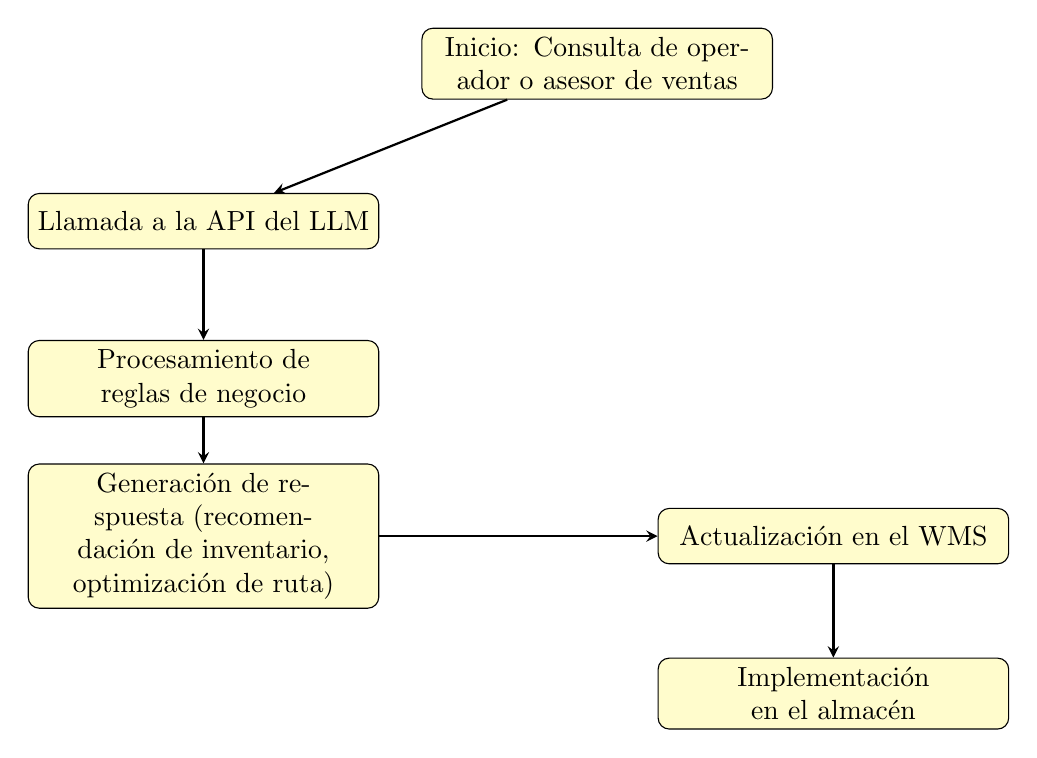
\begin{tikzpicture}[node distance=2cm, auto]
% Styles
\tikzstyle{block} = [rectangle, draw, fill=yellow!20, text centered, rounded corners, minimum height=2em, text width=12em]
\tikzstyle{arrow} = [thick,->,>=stealth]

% Nodes
\node (start) [block] {Inicio: Consulta de operador o asesor de ventas};
\node (api) [block, below of=start, xshift=-5cm] {Llamada a la API del LLM};
\node (rules) [block, below of=api] {Procesamiento de reglas de negocio};
\node (response) [block, below of=rules] {Generación de respuesta (recomendación de inventario, optimización de ruta)};
\node (wms) [block, right of=response, xshift=6cm] {Actualización en el WMS};
\node (final) [block, below of=wms] {Implementación en el almacén};

% Arrows
\draw [arrow] (start) -- (api);
\draw [arrow] (api) -- (rules);
\draw [arrow] (rules) -- (response);
\draw [arrow] (response) -- (wms);
\draw [arrow] (wms) -- (final);
\end{tikzpicture}

\subsection{Beneficios de Integrar LLM con WMS}

La integración de un LLM con un WMS puede traer una serie de beneficios operativos importantes:

\begin{itemize}
    \item **Automatización de reglas de negocio**: Los operadores o asesores virtuales pueden interactuar con el sistema mediante una interfaz que procesa reglas de negocio específicas, como la gestión de inventarios, reabastecimiento y optimización de rutas.
    \item **Mejora en la precisión de las decisiones**: A través del análisis de datos históricos y en tiempo real, el LLM puede mejorar la precisión de las decisiones operativas en el almacén.
    \item **Escalabilidad**: La implementación de un LLM permite escalar operaciones rápidamente sin necesidad de ampliar de manera significativa el equipo de trabajo.
\end{itemize}

\subsection{Evaluación Comparativa: Integración de LLM en WMS a 5 Meses}

A continuación se presenta una tabla comparativa que evalúa los resultados obtenidos al integrar un LLM con un WMS a lo largo de 5 meses, comparado con la contratación de un equipo interno de IA.

\begin{table}[H]
\centering
\caption{Evaluación de Resultados a 5 Meses: Integración de LLM en WMS vs. Equipo Interno de IA}
\resizebox{\textwidth}{!}{
\begin{tabular}{@{}>{\bfseries}l>{\raggedright\arraybackslash}p{5cm}>{\raggedright\arraybackslash}p{5cm}>{\raggedright\arraybackslash}p{5cm}@{}}
\toprule
\textbf{Parámetro} & \textbf{LLM en WMS (5 meses)} & \textbf{Equipo Interno de IA (5 meses)} \\ \midrule
Costo Acumulado & \$50 USD (500 llamadas) & \$10,000 USD (salarios y herramientas) \\
Exactitud & 63\% & Entre 76\% y 87\% \\
Personalización & Limitada (dependencia de la API) & Alta (modelos ajustados a las reglas de negocio específicas) \\
Impacto en el negocio & Resultados rápidos, útiles para prototipos y pruebas & Alta precisión, ideal para entornos de producción \\ \bottomrule
\end{tabular}}
\end{table}

\subsection{Conclusión}

Unir un LLM con un WMS ofrece una solución eficiente para automatizar y mejorar las decisiones operativas en el almacén. Aunque la exactitud y personalización del uso de LLM mediante API puede ser menor en comparación con un equipo de IA interno, el costo y la rapidez de implementación lo hacen una opción atractiva para empresas que buscan resultados inmediatos. Además, esta integración proporciona una base sólida para futuras mejoras, como el desarrollo de interfaces de ventas automatizadas que ayuden a gestionar reglas de negocio en tiempo real.

\begin{figure}[H]
\centering
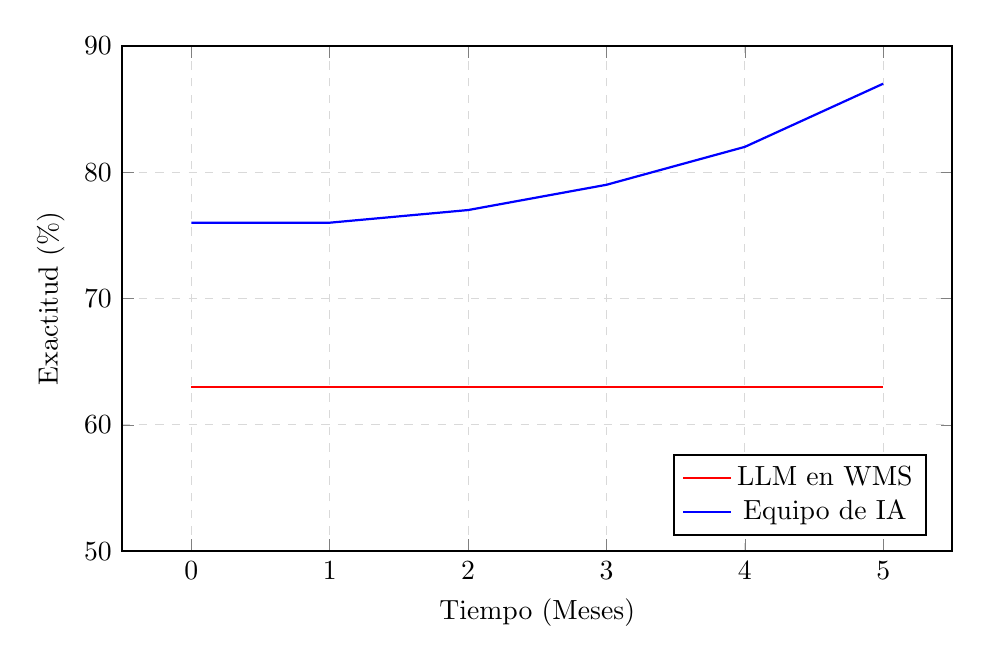
\begin{tikzpicture}
    \begin{axis}[
        width=\textwidth,
        height=8cm,
        grid=both,
        xlabel={Tiempo (Meses)},
        ylabel={Exactitud (\%)},
        legend pos=south east,
        ymin=50, ymax=90,
        grid style={dashed, gray!30},
        xtick distance=1,
        ytick distance=10,
        thick
    ]
    \addplot[color=red, thick] coordinates {
        (0, 63) (1, 63) (2, 63) (3, 63) (4, 63) (5, 63)
    };
    \addplot[color=blue, thick] coordinates {
        (0, 76) (1, 76) (2, 77) (3, 79) (4, 82) (5, 87)
    };
    \legend{LLM en WMS, Equipo de IA}
    \end{axis}
\end{tikzpicture}
\caption{Comparación de Exactitud a lo largo del Tiempo: LLM en WMS vs. Equipo Interno de IA}
\end{figure}
